\textbf{\underline{OZ 4 - De wet van Ampère en de wet van Biot-Savart - Oefening 5:}}
\vspace{0.5cm}

% \vspace{-1cm}

% \begin{minipage}{.73\textwidth}
%     Een lange cilindrische geleider met straal $a$ heeft twee cilindrische gaten van diameter $a$ doorheen zijn hele lengte. Een stroom $I$ vloeit door de geleider en is uit het blad gericht. De stroomdichtheid is uniform doorheen de doorsnede van de draad. Wat is het magnetisch veld in termen van $\mu_0$, $I$, $r$ en $a$ in punt $P_1$? Dezelfde vraag voor punt $P_2$.
% \end{minipage}
% \begin{minipage}{.23\textwidth}
%     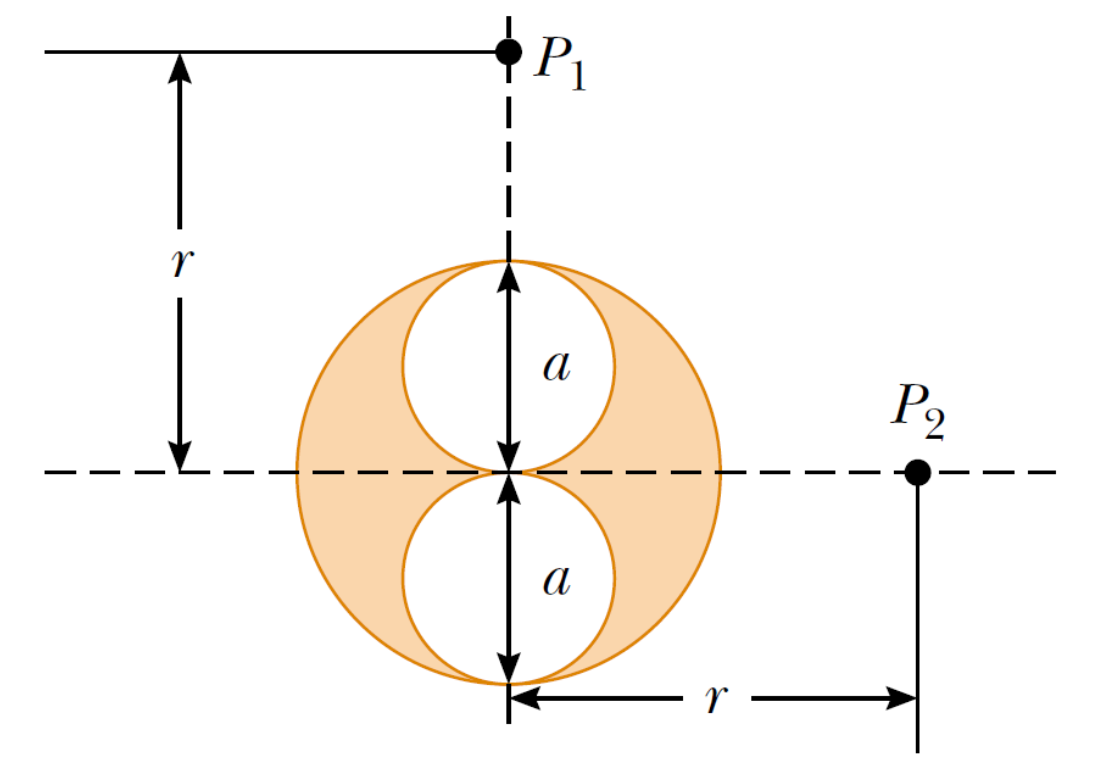
\includegraphics[scale = 0.25]{oz04/resources/Oz4Oef5.png}
% \end{minipage}

Een lange cilindrische geleider met straal $a$ heeft twee cilindrische gaten van diameter $a$ doorheen zijn hele lengte (zie doorsnede in Figuur 5). Een stroom $I$ vloeit door de geleider en is uit het blad gericht. De stroomdichtheid is uniform doorheen de doorsnede van de draad. Wat is het magnetisch veld in termen van $\mu_0$, $I$, $r$ en $a$ in punt $P_1$? Dezelfde vraag voor punt $P_2$.
    
\begin{center}
    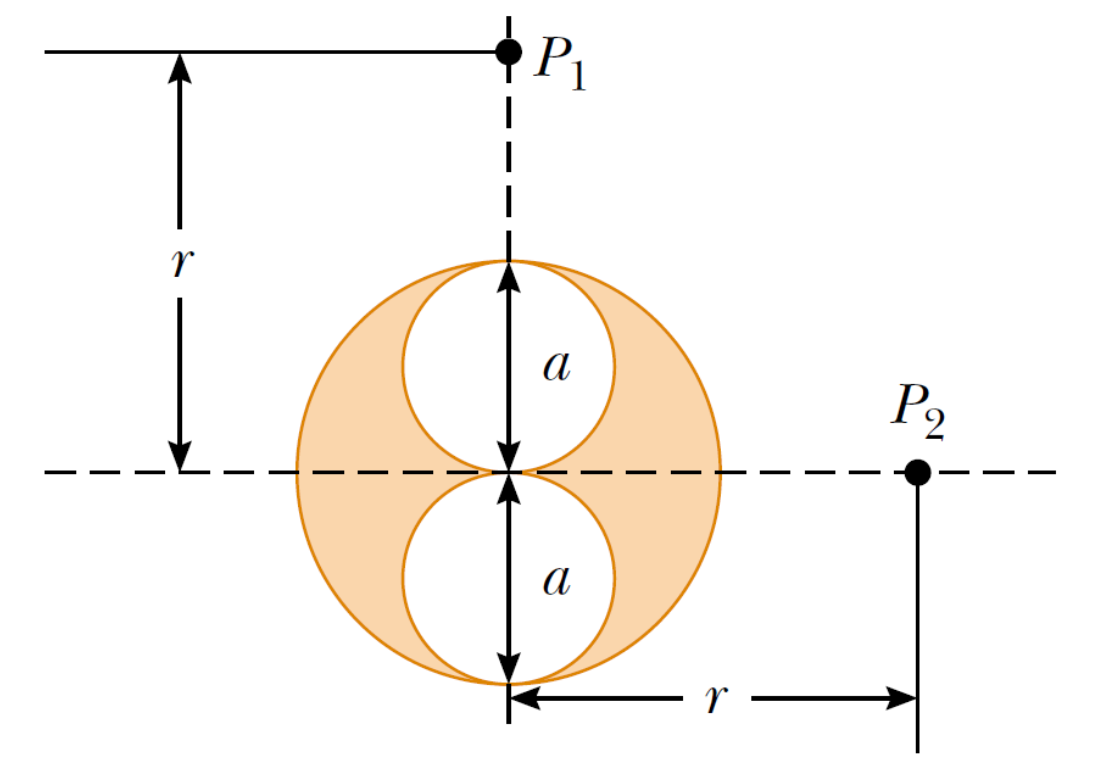
\includegraphics[scale = 0.3]{oz04/resources/Oz4Oef5.png}
\end{center}

% \begin{description}[labelwidth=1.5cm, leftmargin=!]
%     \item[Geg. :]   
%     \item[Gevr. :]  
%     \item[Opl. :]  
% \end{description}

% De oppervlakte is gelijk aan
% \begin{equation*}
%     A = \pi a^2 - 2\pi \left(\frac{a}{2}\right)^2 = \pi \frac{a^2}{2}
% \end{equation*}

\begin{description}[labelwidth=1.5cm, leftmargin=!]
    \item[Opl. :]  
    
        Neem $B_1$ het magnetisch veld door het gekleurde deel, $B_2$ het magnetisch veld door de bovenste caviteit en $B_3$ het magnetisch veld door de onderste caviteit.
        De oppervlakte $A$ waardoor stroom vloeit is
        \begin{equation*}
            A = \pi\left(a^2 - \frac{a^2}{2}\right) = \pi\frac{a^2}{2}
        \end{equation*}
        waaruit volgt dat de stroom dichtheid $J$ het volgende is
        \begin{equation*}
            J = \frac{2I}{\pi a^2}.
        \end{equation*}        
\end{description}

\begin{enumerate}[leftmargin = 0cm,label = \subscript{P}{{\arabic*}}: ]
    \begin{minipage}[t]{.48\textwidth}
        \item 
        \begin{description}[labelwidth=1.5cm, leftmargin=!]
            \item[Geg. :]  $\mu_0$, $I$, $r$, $a$
            \item[Gevr. :] $B$ in $P_1$ ?
            \item[Opl. :]  
            We vinden de volgende magnetische velden
            \begin{align*}
                \vec{B}_1 
                    &= \frac{\mu_0Ja^2}{r} \ (\hat{i}) \\
                \vec{B}_2
                    &= \frac{\mu_0J(\frac{a}{2})^2}{2\left(r - \frac{a}{2}\right)} \ (-\hat{i}) \\
                \vec{B}_3 
                    &= \frac{\mu_0J(\frac{a}{2})^2}{2\left(r + \frac{a}{2}\right)} \ (-\hat{i})
            \end{align*}
            het totale veld in $P_1$ is
            \begin{align*}
                \vec{B} 
                    &= \sum_{i=1}^3 B_i \ (\hat{i}) \\
                    &= \frac{\mu_0Ja^2}{2} \left[\frac{1}{r} - \frac{1}{4\left(r - \left(\frac{a}{2}\right)\right)} - \frac{1}{4\left(r + \left(\frac{a}{2}\right)\right)} \right] \ (\hat{i}) \\
                    &= \frac{\mu_0I}{\pi r}\left(\frac{2r^2-a^2}{4r^2-a^2}\right) \ (-\hat{i}).
            \end{align*}
        \end{description}    
    \end{minipage}%
    \begin{minipage}[t]{.48\textwidth}
        \item 
        \begin{description}[labelwidth=1.5cm, leftmargin=!] 
            \item[Geg. :]  $\mu_0$, $I$, $r$, $a$
            \item[Gevr. :] $B$ in $P_2$ ?
            \item[Opl. :]  
            We vinden de volgende magnetische velden
            \begin{align*}
                \vec{B}_1 
                    &= \frac{\mu_0Ja^2}{2r} \ (\hat{j}) \\
                \vec{B}_{2,3} 
                    &=  \frac{\mu_0J(\frac{a}{2})^2}{2 \sqrt{r^2 + \left(\frac{a}{2}\right)^2}} \ (-\hat{j})
            \end{align*}
            waarbij $B_{2,3} = B_2 = B_3$. De horizontale componenten van $B_2$ en $B_3$ doen elkaar te niet, het totale veld in $P_2$ is
            \begin{align*}
                \vec{B} 
                    &= \sum_{i=1}^3 B_i \ (\hat{j}) \\
                    % &= \frac{\mu_0Ja^2}{2r} - \left(\frac{\mu_0J(\frac{a}{2})^2}{\sqrt{r^2 + \left(\frac{a}{2}\right)^2}}\frac{r}{\sqrt{r^2 + \left(\frac{a}{2}\right)^2}}\right) \ (\hat{j}) \\
                    &= \frac{\mu_0Ja^2}{2r}\left[1 - \frac{r^2}{2\left(r^2 + \left(\frac{a}{2}\right)^2\right)}\right] \ (\hat{j}) \\
                    &=\frac{\mu_0I}{\pi r}\left(\frac{2r^2+a^2}{4r^2+a^2}\right) \ (\hat{j}).
            \end{align*}
        \end{description}
   \end{minipage}%
\end{enumerate}

\vspace{1cm}